\documentclass[a4paper]{article}

\usepackage[francais]{babel}
\usepackage[utf8]{inputenc}
\usepackage{amsmath}
\usepackage{amssymb}
\usepackage[pdftex]{graphicx}
\usepackage{url}
\usepackage{subfigure}

% shorten margin
\usepackage[]{fullpage}

\title{FUGU : Find Your Guest Unisonously\\Site de covoiturage}
\author{Mathieu BIVERT, Sophie VALENTIN}

\makeatletter
\def\thickhrulefill{\leavevmode \leaders \hrule height 1pt\hfill \kern \z@}
\def\maketitle{%
  \null
  \thispagestyle{empty}%
  \vskip 1cm
  \begin{center}
        \normalfont\large\huge\@author
  \end{center}
  \vfil
  \vfil
  \vfil
  \vfil
  \vfil
  \vfil
  \vfil
  \vfil
  \vfil
  \vfil
  \vfil
  \vfil  
  \vfil  
  \hrule height 2pt
  \par
  \begin{center}
        \huge \strut Projet WASP\\
        \@title \par
  \end{center}
  \hrule height 2pt
  \par
  \vfil
  \vfil
  \vfil
  \vfil
  \vfil
  \vfil
  \vfil
  \begin{figure}[!ht]
  	\centering
  	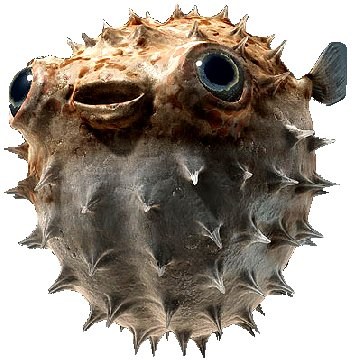
\includegraphics[scale=1]{imgs/fugu_rapport.jpg}
  \end{figure}
  \vfil
  \vfil
  \vfil
  \vfil  
  \vfil  
  \vfil
  \vfil  
  \vfil  
  \vfil
  \vfil
  \vfil
  \vfil
  \vfil
  \vfil
  \begin{center}
  			\huge Professeur : Tamara REZK
  \end{center}
  \null
\cleardoublepage
}
\makeatother

\begin{document}
\maketitle

\newpage

\section{Fonctionnalités de l'application web}

L'utilisateur souhaitant faire du covoiturage doit tout d'abord s'authentifier.
En effet, les utilisateurs possèdent leurs propres données.
L'utilisateur s'authentifie via un formulaire de connexion, illustré dans la
figure \ref{login}. Il doit renseigner son login et son mot de passe.
S'il n'en possède pas, il peut s'enregistrer sur la page d'inscription, en cliquant
sur le lien \og register \fg.

\begin{figure}[!ht]
	\centering
	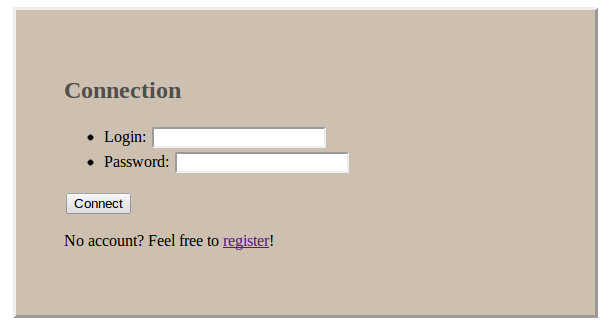
\includegraphics[scale=0.4]{Connexion.png}
	\caption{\label{login} Formulaire de connexion}
\end{figure}

\subsection{Tableau de bord de gestion}

Une fois authentifié, l'utilisateur accède à son tableau de bord, représenté en
figure \ref{dashboard}. Cet écran répertorie tous ses trajets, c'est-à-dire les
trajets dont il est le:
\begin{description}
	\item[conducteur], dans la partie haute de la page;
	\item[passager], dans la partie basse de la page.
\end{description}

\begin{figure}[!ht]
	\centering
	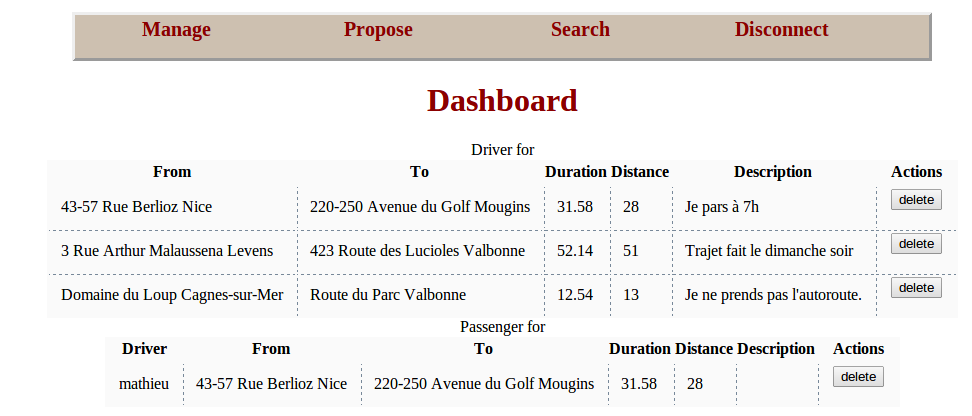
\includegraphics[scale=0.5]{Dashboard.png}
	\caption{\label{dashboard} Tableau de bord}
\end{figure}

L'utilisateur a accès à tout moment à ce tableau de bord en cliquant
sur \og Manage \fg\ dans le menu de navigation. Enfin, il peut se
déconnecter en cliquant sur \og Disconnect \fg.

\begin{figure}[!ht]
	\centering
	
\includegraphics[scale=0.4]{Menu.png}
	\caption{\label{menu} Menu de navigation}
\end{figure}

\newpage

Pour chaque trajet, les adresses de départ et d'arrivée sont affichées.
Le temps (en minutes) et la distance (en kilomètres), qui ont été calculés,
sont également affichés. L'utilisateur peut voir la description qui a été
donnée au trajet. Généralement, ce sont des informations pratiques sur
le rendez-vous.

L'utilisateur peut supprimer un trajet de son tableau de bord : pour cela,
il clique sur le bouton \og delete \fg du trajet qu'il souhaite supprimer.
Son tableau de bord est alors mis à jour. S'il était conducteur pour ce
trajet, alors le trajet n'apparaîtra plus dans le tableau de bord des
autres passagers. 

\subsection{Proposition de trajet}

En cliquant sur \og Propose \fg sur le menu de navigation, l'utilisateur peut
proposer un trajet comme dans la figure \ref{propose}. Au chargement,
une carte apparaît avec une adresse de départ et une adresse d'arrivée
par défaut. Pour indiquer son trajet, l'utilisateur a deux solutions 
:
\begin{itemize}
	\item il peut entrer les adresses de départ et destination dans les champs
	\item il peut déplacer les marqueurs sur la carte
\end{itemize}

Dans le premier cas, les marqueurs sur la carte sont immédiatement mis à jour.
Dans le second cas, les champs d'adresses sont immédiatement mis à jour.
Et quelque soit la méthode pour indiquer le trajet, le temps de trajet
et la distance sont calculées. L'utilisateur a ensuite la possibilité de
laisser une description en remplissant le champ de texte.
Pour terminer, il enregistre son trajet en cliquant sur le bouton
\og Propose \fg, en-dessous de la description.

\begin{figure}[!ht]
	\centering
	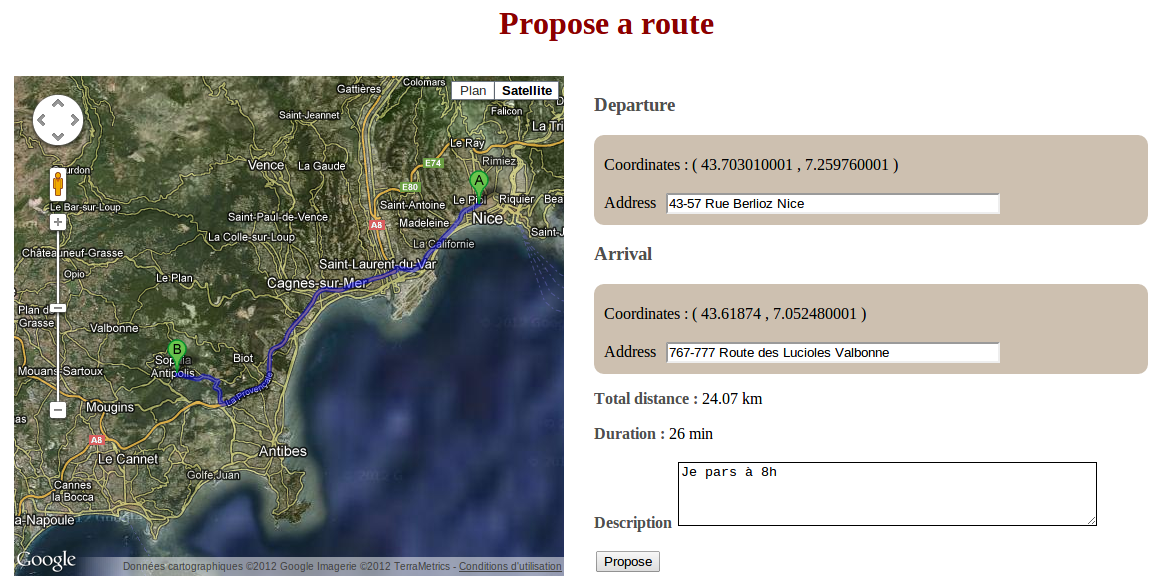
\includegraphics[scale=0.4]{Propose.png}
	\caption{\label{propose} Proposition de trajet}
\end{figure}

Après enregistrement, l'utilisateur est redirigé sur le tableau de
bord où apparaît alors le trajet nouvellement créé.

\subsection{Recherche de trajet}

En cliquant sur \og Search \fg sur le menu de navigation, l'utilisateur
peut chercher un trajet existant. Le principe est le même que pour la création
de trajet à l'exception que l'utilisateur ne renseigne aucun champ de description.
Après un clic sur le bouton \og Search \fg, une liste de trajets est affichée. 

\begin{figure}[!ht]
	\centering
	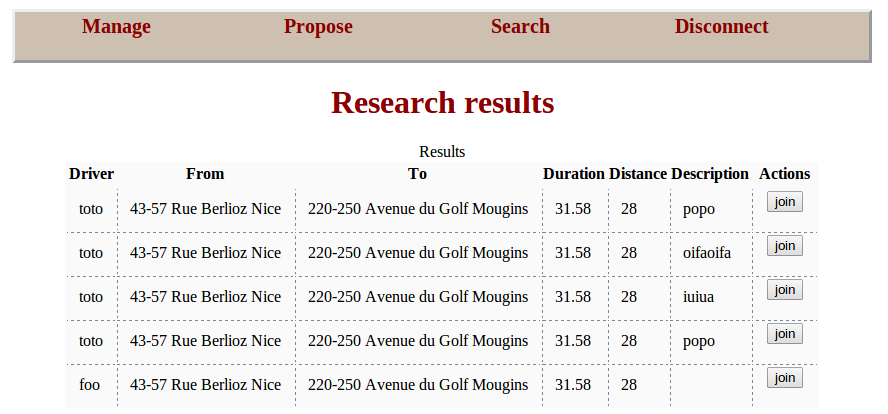
\includegraphics[scale=0.5]{Search.png}
	\caption{\label{search} Recherche de trajet}
\end{figure}
\newpage

Pour chaque trajet, on peut s'inscrire en tant que passager. Il faut
noter que les trajets sur lesquels on s'est déjà inscrit ne figurent
pas dans la recherche. Pour s'inscrire, on clique sur le bouton \og join \fg
en face du trajet. On est alors redirigé vers le tableau de bord où apparaît
maintenant le trajet que l'on a rejoint.

\section{Serveur}
\subsection{Services}

Les différentes pages fournissent les services suivants:
\begin{description}
	\item[index.php] connexion;
	\item[register.php] inscription;
	\item[user.php] listes des trajets de l'utilisateur;
	\item[proposer\_trajet.php] enregistrer un nouveau trajet;
	\item[chercher\_trajet.php] chercher un trajet existant;
	\item[lister\_trajets.php] lister les trajets existants;
	\item[disconnect.php] déconnexion;
\end{description}

\subsection{Securité}
\subsubsection{Prévention de l'attaque XSRF}
 		
Une telle attaque envoie des requêtes à l'insu de l'utilisateur
depuis son propre navigateur. Pour la contrer, on génère sur
chaque page un jeton (ou token), qui est stocké côté serveur,
avec la fonction PHP  \textit{openssl\_random\_pseudo\_bytes()},
qui est un générateur pseudo-aléatoire d'octets.

Pour obtenir un service habituel, il faut préciser, selon les pages, en mode GET
ou en mode POST le token obtenu. Le serveur vérifie que le paramètre
(GET ou POST) est bien égal au token stocké côté serveur.
Ainsi, si l'attaquant tente d'envoyer une requête sans connaître le
token et la façon d'envoyer le paramètre, il n'obtiendra pas le service.

Par exemple, pour le service de proposition de trajet, la comparaison entre
le token mis en mémoire sur le serveur et celui passé en paramètre se fait
dans le fichier \textit{proposer\_trajet.php:54}. Sur cette ligne, on appelle en
fait la fonction \textit{compare\_token\_with()} définie dans le fichier
inc/xsrf.php. Quant à la génération du nouveau token, elle se fait dans
\textit{proposer\_trajet.php:57}.  Sur cette ligne, on appelle la fonction
\textit{generate\_token()} définie dans le fichier \textit{inc/xsrf.php}.
 		
Le fait de regénérer le token à chaque requête est gênant si on
souhaite ouvrir deux onglets par exemple. En effet, l'une des deux
pages ouvertes modifie le token enregistré côté serveur et pour l'autre
page, la vérification échouera à cause de la désynchronisation.
Un autre moyen de prévenir XSRF peut être de générer un token par
session pour éviter ce genre de désagréments mais cette façon de faire
est moins sûre.
 		
\subsubsection{Prévention des attaques contre l'intégrité de la session}
On souhaite éviter que l'utilisateur puisse modifier les données sensibles fournies par le serveur : 
celles-ci peuvent être stockées par exemple dans les cookies ou dans les champs hidden. 
Pour ce faire, on stocke côté serveur une empreinte
HMAC de ces données. Cette empreinte est
calculée grâce à deux entrées:

\begin{itemize}
	\item la donnée que l'on souhaite passer à l'utilisateur ;
	\item la clé privée connue seulement du serveur.
\end{itemize}

Lors de l'envoi de données altérées,
le serveur détectera que l'empreinte de la donnée envoyée par le client
n'est pas la même que celle stockée côté serveur. Ainsi on prévient les
attaques visant à altérer les données de session.

Dans notre cas, l'utilisation des cookies est restreinte à l'ID de session.
Quant aux champs hidden, on les utilise uniquement pour des informations non
sensibles.
\begin{itemize}
	\item Tout d'abord, ils sont utilisés pour des actions prédéfinies sur le serveur. 
	Ainsi, si on fournit des actions inexistantes, le code ne fera aucun traitement.
	\item Ensuite, ils sont utilisés pour maintenir les informations sur la distance
	et sur le temps de trajet. Ces informations sont calculées dynamiquement sur les données
	du trajet de l'utilisateur par le Javascript (API Google Maps). Par conséquent, 
	le stockage d'un HMAC côté serveur nous semblait compromis dans le sens où le
	client peut modifier ces informations dès qu'elles sont calculées. 
	De plus, ces informations ont un niveau de sécurité bas et n'entravent pas
	le bon fonctionnement de l'application basée sur les points de départ et d'arrivée. 
	Dans l'idéal, il faudrait recalculer le temps et la distance du trajet côté serveur.
\end{itemize}

\subsubsection{Prévention des attaques de fixation}
Pour une telle attaque, l'attaquant fixe le Session ID dans l'URL pour
un autre utilisateur. Il envoie ensuite cette URL à l'utilisateur. Ce
dernier s'authentifie et l'attaquant peut alors utiliser la session de
l'utilisateur car il connait le SID. Pour prévenir cette attaque, il faut
modifier le fichier \textit{php.ini} du serveur :

\begin{itemize}
	\item en activant l'option \textit{session.use\_only\_cookies} afin que
		le SID soit transmis exclusivement par cookie ;
	\item en s'assurant que l'option \textit{session.use\_trans\_sid} est désactivée. 
	En la désactivant, on s'assure que les SID ne sont pas transmis par la méthode GET.
\end{itemize}

\subsubsection{Prévention des attaques Man in the Middle}
Pour réduire la probabilité d'une attaque de type MiM, on utilise un flux
chiffré tel que HTTPS. Cela nous assure les propriétés de confidentialité
et d'intégrité des paquets transmis.

EXPLIQUER DEPLOIEMENT HTTPS

\subsubsection{Prévention des \og Replay Attacks \fg}
Les replay attacks permettent à un attaquant d'envoyer plusieurs fois un
même paquet (eg. celui de connexion).

Comme la protection des failles CSRF/XSRF intègre la génération d'un
token à chaque nouvelle action de l'utilisateur, la retransmission d'un
même paquet est impossible.

\subsubsection{Prévention des attaques XSS}
 		
Cette attaque utilise le navigateur du client. Du code d'un domaine qui
n'est pas de confiance est interprété dans le navigateur du client.
Il peut s'agir d'une redirection forcée pour faire  du phising
ou d'un vol de cookie avec du Javascript.

Pour protéger le vol de cookie, on active l'option \textit{session.cookie\_httponly}
dans le fichier \textit{php.ini}. Cela permet de rendre les cookies HttpOnly,
c'est-à-dire qu'ils ne seront pas accessibles par des langages de script
tels que Javascript. Il faut également vérifier les données utilisateur
comme dans le cas des attaques d'injections de code en retraitant le code
HTML produit. Pour ce faire, on appelle la fonction \textit{hmlspecialchars}.
 		
\subsubsection{Prévention des attaques d'injection de code}
La prévention des attaques d'injection de code passe par :
\begin{itemize}
	\item une identification précise des entrées qui ne sont pas de
		confiance pour ensuite s'assurer que ces données ne sont pas
		considérées avec un niveau de sécurité plus haut dans le code
		(taint analysis) 
	\item un assainissement des entrées
\end{itemize}
		
\paragraph{Injections SQL}
~~\\
\\
Il faut vérifier les données de l'utilisateur et échapper les caractères spéciaux.
Dans notre cas, nous utilisons des requêtes préparées en PHP.
Tout d'abord, on écrit une requête à trous sans les paramètres. Ensuite, la
requête est analysée et compilée. Enfin, les paramètres sont donnés et le driver
SQLite pour PHP gère automatiquement l'échappement des caractères spéciaux.
Concernant la vérification, elle est faite en utilisant des expressions régulières.			
Par exemple, on vérifie un format raisonable pour les addresses emails dans
\textit{inc/utils.php:38}.

Par exemple pour tester si un utilisateur existe, on prépare la requête
dans \textit{inc/user.php:19}, puis on l'exécute \textit{inc/user.php:25}.

\paragraph{Injections Javascript}
~~\\
\\
On veut éviter qu'un utilisateur insère un script Javascript dans un champ.
Pour pallier ce problème, on transforme les caractères spéciaux du texte entré afin
qu'un éventuel script Javascript deviennent du texte non interprété.
Pour cela, on utilise la fonction sanitized d'\textit{inc/utils.php}. Cette fonction
appelle la fonction PHP \textit{htmlspecialchars()}, \textit{inc/utils.php:124}.
		
\subsubsection{Prévention des attaques RFI/LFI}
		
\paragraph{RFI}
~~\\
\\
On ne fait pas de include en PHP en utilisant les données utilisateur.
L'utilisateur ne peut pas nous forcer à inclure un fichier important du serveur.
Cela nous protège des attaques LFI.

\paragraph{LFI}
~~\\
\\
On n'inclut pas d'URL externe dans le code PHP.
Par sécurité dans le fichier php.ini, on désactive l'option \textit{allow\_url\_include} 
Cela nous protège des attaques RFI.

\subsubsection{Prévention des attaques par distingueur}
On utilise des systèmes de hashage \og robustes \fg, par exemple, on
préfère SHA à MD5. Le générateur de nombre aléatoire utilisés est \textit{/dev/random}
sous UNIX: en effet, bien que plus long que son homologue \textit{/dev/urandom},
il fournit des nombres \og plus \fg\ aléatoires.
		
\subsubsection{D'autres éléments de prévention}

Pour limiter les vols de cookies, lors d'une déconnexion, les cookies sont
effacés de la machine ciente. Cela permet, par exemple, de limiter des vols
causés par une intrusion sur le disque dur de utilisateur.

Au niveau du déploiement, le serveur HTTP peut-être placé dans un environnement
virtualisé (VM), ou pseudo-virtualisé (chroot, BSD jail) pour éviter de compromettre
le système hôte en cas de défaillance au niveau du serveur comme du code du site
web.

Une protection basique contre les attaques de type \textbf{DDoS} est faisable en
utilisant des modules comme \textit{mod\_evasive} ou \textit{mod\_slotlimit} dans
le cadre d'un déploiement sous apache$2$.

Les mots de passes sont hashés (\textit{hash('sha512', \$password)}) avant d'être
stockés dans la base de données. Cela évite une divulgation des mots de passe si
le contenu de la bdd venait à être compromis, ce qui est une bonne idée lorsque
un utilisateur utilise le même mot de passe pour plusieurs comptes sur Internet.

\section{Client}
\subsection{Google Maps}

Pour dialoguer avec le mashup intégré dans la page, on utilise l'API Google Maps.

\subsubsection{Carte, coordonnées et adresses}

\paragraph{Service \textit{Geocode}}
~~\\
\\
Tout d'abord, on utilise le type Map pour obtenir le mashup et le lier à un élément 
de notre page.
Et on utilise le service Geocode de Google qui permet de traduire 
des adresses en coordonnées et inversement.
Par exemple, dans \textit{js/carte.js:8}, il y a création d'un objet \textit{Geocode} 
et appel de la fonction \textit{geocode()}. On définit une fonction de callback pour 
la réponse du service où on peut alors accéder au résultat de la traduction.

\paragraph{Type \textit{LatLng}}
~~\\
\\
Les points (coordonnées) sont représentés par le type \textit{LatLng}.
On l'utilise notamment pour définir le point de centre de la carte
au chargement et ensuite, pour définir les coordonnées des points
de départ et d'arrivée.

\subsubsection{Calcul des itinéraires}

\paragraph{Service \textit{DirectionsService}}
~~\\
\\
On utilise le service \textit{DirectionsService}.
Effectivement, pour calculer les données de l'itinéraire (temps et distance), 
on a besoin que l'API de Google détermine les différents segments de 
l'itinéraire. Ainsi, on appelle la fonction \textit{route()} 
de \textit{DirecionsService} où on spécifie :
- les coordonnées de départ ;
- les coordonnées d'arrivée ;
- le moyen de locomotion (ici voiture).
On définit là aussi une fonction de callback pour la réponse.
Un exemple d'appel est disponible dans \textit{js/carte.js:91}
On obtient dans le résultat de la réponse de type \textit{DirectionsResult} 
différents tableaux. Par exemple, on obtient
un premier tableau avec des points (coordonnées) appartenant à l'itinéraire
calculé. On obtient également un tableau avec des segments de l'itinéraire.
Le second tableau nous sert à calculer la distance totale et le temps total
car chaque segment contient une information sur son temps et sa distance. 
Voir la fonction \textit{calculerDistanceEtTemps} dans \textit{js/carte.js:29}).

\paragraph{Synchronisation sur la carte}
~~\\
\\
Quant à l'objet \textit{DirectionsRenderer}, il nous permet de synchroniser sur l'objet
\textit{Map} l'itinéraire calculé de type \textit{DirectionsResult}. C'est cet objet
qui affiche l'itinéraire en bleu sur la carte.
Ainsi, à chaque réponse de la méthode \textit{route()}, on met à jour l'information
d'itinéraire \textit{DirectionsResult} dans l'objet \textit{DirectionsRenderer} pour que
l'affichage de la carte soit modifié et bien entendu, on calcule les informations
de distance et de durée. Cela est fait à chaque fois que l'utilisateur modifie
les champs d'adresse dans le formulaire. 

\paragraph{Utilisation d'un listener}
~~\\
\\
Mais il faut également que les actions de l'utilisateur sur la carte soient prises en compte.
En effet, un déplacement des marqueurs ou un déplacement de l'itinéraire en bleu doit
provoquer une mise à jour des marqueurs, des adresses dans les champs du formulaire,
et des données de l'itinéraire comme la distance et le temps. Pour cela,
un évènement est créé : l'objet \textit{DirectionsRenderer} écoute les modifications sur la carte.

\subsection{Javascript}

\subsubsection{Utilisation de la Prototype Chain}
Javascript est un langage orienté objet à prototype. Ce dernier point
le différencie des langages objets dits à classes (Smalllalk, Java, etc.).

En js, un objet possède une référence à un autre objet appelé son prototype.
Celui-ci permet de mettre en place une relation d'héritage.

Supposons la relation de prototype suivante : on définit $a$ comme une variable
contenant un champ entier $v$ de valeur $1$, puis $b$ comme un objet dont
le protoype est l'objet $a$:
\begin{verbatim}
js> var a = {v: 1};
js> var b = Object.create(a);
\end{verbatim}

Lorsque l'on essaye d'accéder à une propriété de $b$, la chaîne de prototype
est remontée jusqu'à trouver ladite propriété:
\begin{verbatim}
js> b.v
1
js> b.baz
js>
\end{verbatim}

Dans le premier cas, aucun champs $v$ n'existe dans $b$; on regarde donc
dans son prototype, où l'on trouve bien ce champ. Dans le second, ni $b$
ni $a$ ne contiennent de champ $baz$. On remonte donc au protoype de $a$,
qui est inexistant (plus exactement, il vaut $null$). Aucune valeur n'est
donc retournée.

L'exemple suivant permet de s'assurer que la relation de prototype fonctionne
bien sur des objets (et pas sur des interfaces par exemple):
\begin{verbatim}
js> a.v = 5
5
js> b.v
5
/*
 * ici, on ne remonte pas la chaîne de prototype : un nouveau champ
 * v est crée dans b.
 */
js> b.v = 42
42
js> a.v
5
/*
 * certaines implémentations de javascript permettent d'accèder au
 * prototype d'un objet via la notation non standard __proto__:
 */
js> b.__proto__.v = 42
42
js> a.v
42
\end{verbatim}

\subsubsection{Utilisation de la Scope Chain}

La règle de la scope chain est la suivante :
Si une propriété n'est pas trouvée dans le contexte de l'objet courant,
alors une recherche est lancée dans l'objet parent, et ainsi de suite
jusqu'à éventuellement atteindre l'objet \textit{global}. 

On utilise par exemple la variable \textit{coordonneesDepart}, qui est en
 fait une propriété de l'objet \textit{global}, dans la fonction \textit{init} 
 (\textit{js/carte.js:66}). 
La définition de cette fonction est un objet. Ainsi, 
quand on utilise la variable \textit{coordonneesDepart} dans cette fonction,
on cherche s'il existe une propriété définie dans l'objet courant
(la fonction).
Comme ce n'est pas le cas, on remonte la scope chain d'un cran et on trouve
la propriété \textit{coordonneesDepart} dans l'objet \textit{global}.

\subsubsection{Utilisation du mot-clé this}

Le mot-clé \textit{this} est une propriété du contexte d'exécution.
Le mot-clé \textit{this} est donc une référence vers l'objet \textit{global} sauf
dans certains cas. Par exemple, si \textit{this} est utilisé dans une fonction,
alors la valeur de \textit{this} dépend du contexte d'exécution lors de l'appel
de la fonction. 

Nous utilisons le mot-clé \textit{this} par exemple dans \textit{proposer\_trajet.php:98}.
La valeur de \textit{this} est ici \textit{global}.

\subsubsection{Utilisation de la récursivité}

Nous utilisons des structures de contrôle de type boucle for, par exemple
dans \textit{proposer\_trajet.php:37}.

\subsubsection{Manipulation du DOM}

L'accès aux éléments de la page HTML se base sur l'id des balises et se fait dans le Javascript
avec \textit{document.getElementById()}.
Des manipulations du DOM sont effectuées depuis le Javascript.
En effet, on modifie par exemple la valeur de champs hidden dans \textit{proposer\_trajet.php:45}.
Ou encore, on remplace le contenu d'une balise dans \textit{proposer\_trajet.php:44}.

\subsection{Securité} 

\subsubsection{Prévention des failles Javascript}

Concernant la sécurité, l'objet \textit{global} ne doit pas être délivré
à l'attaquant puisque l'intégralité de la page y est accessible. De plus,
on peut y trouver les cookies. 

On a donc vu dans la deuxième partie de ce rapport, qu'il fallait prévenir
les attaques de type XSS et injection de code.

Ici, du code extérieur est inclus. On utilise le mashhup avec la balise \textit{script}.
Or, en utilisant \textit{script}, la mémoire de la page intégrant le mashup et la mémoire du mashup 
ne sont pas scindées : l'objet \textit{global} est partagé. Le code du script inclus peut donc accéder
à l'objet \textit{global}.

Une alternative pour intégrer un tel mashup serait d'utiliser la balise \textit{iframe} pour avoir
des mémoires séparées. Cependant, il faudrait mettre en place un mécanisme de communication entre les deux
parties avec \textit{postMessage}.

Cependant, le code intégré ici provient de Google, qui est considéré comme un domaine de confiance.

\newpage
\appendix
\section{php.ini}
On donne ici un extrait d'un \textit{php.ini} pouvant être
utilisé par notre application.

\begin{verbatim}
; don't give unecessary informations about PHP
expose_php = Off

; restrict execution and input processing time
max_execution_time = 30
max_input_time = 60

; limit the memory used by a script
memory_limit = 128M

; report every error and log them
error_reporting = E_ALL
log_errors = On
log_errors_max_len = 1024
report_memleaks = On
; no need for pretty error messages
html_errors = Off

; don't give unecessary debug informations to users
display_errors = Off
display_startup_errors = Off

; default mimetype and charset
default_mimetype = "text/html
default_charset = "UTF-8"

[Session]
; use files to store/retrieve session data
session.save_handler = files
session.save_path = "/var/lib/php"

; do use cookie, secure cookie
session.use_cookies = 1
session.cookie_secure = 1
; store session ID in cookie
session.use_only_cookies = 1
session.name = PHPSESSID

; cookie unavailable from js
session.cookie_httponly = 1

; use /dev/random over /dev/urandom as an entropy generator
; slower but more resistant to statistical attacks
session.entropy_file = /dev/random

; avoid sending SID within an URL
session.use_trans_sid = 0

; 1 : SHA-1 (160b), 0 : MD5 (128b)
session.hash_function = 1
\end{verbatim}

\end{document}
